\documentclass[border=5pt]{standalone}
\usepackage[T1]{fontenc}
\usepackage[utf8]{inputenc}
\usepackage{amsmath}
\usepackage{graphicx}
\usepackage{tikz}
\usetikzlibrary{positioning,arrows.meta,calc,shapes.geometric}

\begin{document}
\resizebox{150mm}{!}{%
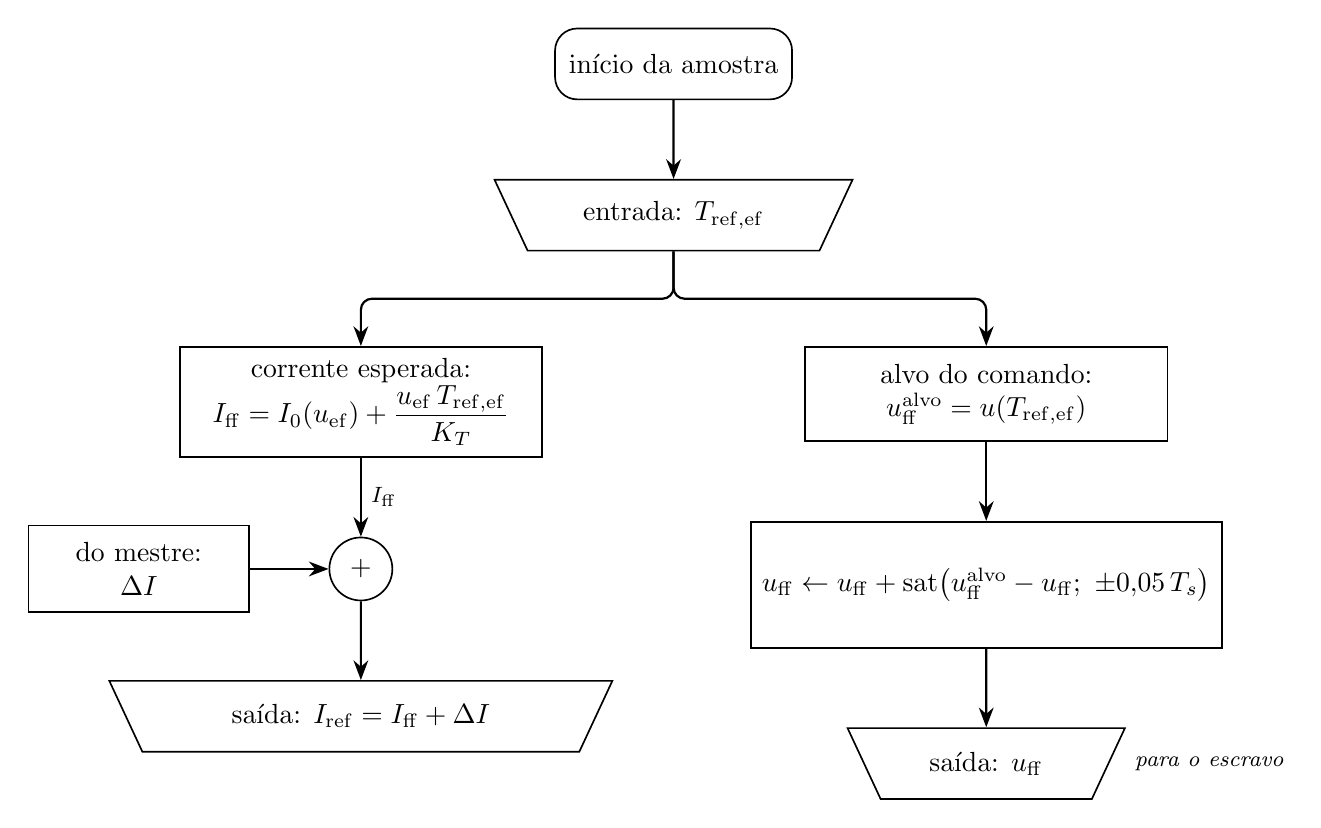
\begin{tikzpicture}[
  font=\normalsize,
  term/.style={draw=black, semithick, rounded corners=8pt, minimum height=9mm, inner sep=5pt, align=center},
  block/.style={draw=black, semithick, minimum height=12mm, minimum width=46mm, inner sep=4pt, align=center},
  io/.style={draw=black, semithick, trapezium, trapezium angle=65, shape border rotate=180, minimum height=9mm, inner sep=4pt, align=center},
  sum/.style={circle, draw=black, semithick, minimum size=8mm, inner sep=0pt},
  lab/.style={font=\footnotesize\itshape},
  arr/.style={-{Stealth[length=2.5mm]}, thick},
  node distance=10mm]
\node[term] (ini) {início da amostra};
\node[io, below=of ini] (ent) {entrada: $T_{\mathrm{ref,ef}}$};
% ramo esquerdo: feedforward de corrente + somador
\node[block, below left=12mm and 12mm of ent] (iff) {corrente esperada:\\$I_{\mathrm{ff}} = I_0(u_{\mathrm{ef}}) + \dfrac{u_{\mathrm{ef}}\,T_{\mathrm{ref,ef}}}{K_T}$};
\node[sum, below=of iff] (soma) {$+$};
\node[block, left=of soma, minimum width=28mm, minimum height=11mm] (di) {do mestre:\\$\Delta I$};
\node[io, below=of soma] (saida) {saída: $I_{\mathrm{ref}} = I_{\mathrm{ff}} + \Delta I$};
% ramo direito: comando equivalente com rampa propria
\node[block, below right=12mm and 12mm of ent] (alvo) {alvo do comando:\\$u_{\mathrm{ff}}^{\mathrm{alvo}} = u\!\left(T_{\mathrm{ref,ef}}\right)$};
\node[block, below=of alvo, minimum height=16mm] (rampa) {$u_{\mathrm{ff}} \leftarrow u_{\mathrm{ff}} + \mathrm{sat}\!\left(u_{\mathrm{ff}}^{\mathrm{alvo}} - u_{\mathrm{ff}};\ \pm 0{,}05\,T_s\right)$};
\node[io, below=of rampa] (saidauff) {saída: $u_{\mathrm{ff}}$};
\node[lab, anchor=west] at ($(saidauff.east)+(2mm,0)$) {para o escravo};
\draw[arr] (ini) -- (ent);
\draw[arr, rounded corners] (ent.south) -- ++(0,-6mm) -| (iff.north);
\draw[arr, rounded corners] (ent.south) -- ++(0,-6mm) -| (alvo.north);
\draw[arr] (iff) -- node[lab, right] {$I_{\mathrm{ff}}$} (soma);
\draw[arr] (di) -- (soma);
\draw[arr] (soma) -- (saida);
\draw[arr] (alvo) -- (rampa);
\draw[arr] (rampa) -- (saidauff);
\end{tikzpicture}}
\end{document}
